% Generated by make_artifacts.py from output/results.json
\documentclass[12pt]{article}
\makeatletter
\def\input@path{{../../templates/}{../../../templates/}}
\makeatother
\usepackage{cumcm-paper}
\graphicspath{{output/}{./}}

\begin{document}
\cumcmtitle{基于视线锥包络与分层进化搜索的烟幕干扰弹投放策略}

\begin{abstract}
针对无人机烟幕干扰弹的时空协同投放问题，本文建立导弹、无人机、干扰弹和烟幕云团的统一三维运动模型，并以导弹至圆柱形真目标完整可视边界的视线段均与烟幕有效球相交作为严格遮蔽判据。该判据保留了题目给定的目标半径与高度信息，并以遮蔽时间集合的测度处理多枚烟幕弹造成的不连续遮蔽。

对于问题一，由确定性轨迹计算得到完整圆柱边界的有效遮蔽区间为 8.056--9.448 s，时长 1.392 s；若仅检验目标中心视线则为 1.435 s，说明忽略目标尺寸会高估结果。

对于问题二，将待优化起爆点参数化为导弹--目标中心视线上的点，并由几何关系反求无人机航向、速度和引信时序，再用差分进化搜索。所得航向 176.91$^\circ$、速度 71.00 m/s、投放时刻 0.009 s、起爆时刻 2.461 s，严格遮蔽时长为 4.540 s。

对于问题三，以同一航向和速度约束下的边际遮蔽增益依次安排三枚弹，联合遮蔽 4.620 s；对于问题四，三架无人机采用边际协同搜索，形成三个不连续区间，合计 11.530 s。对于问题五，先比较无人机--导弹配对的可达遮蔽能力，再在各架无人机固定航迹上追加具有正边际收益的烟幕弹。最终使用 8 枚弹，对 M1、M2、M3 分别遮蔽 13.400 s、3.770 s、3.730 s，总和为 20.900 s。全部策略已写入官方 Excel 模板。
\end{abstract}
\keywords{烟幕干扰；视线遮蔽；空间几何；差分进化；协同优化}

\section{问题重述}

三枚导弹以 300 m/s 的速度分别由给定初始位置直线飞向原点处的假目标。半径 7 m、高 10 m 的圆柱形真目标位于其后方，五架无人机可在接令时瞬时改变航向，随后以 70--140 m/s 的恒定速度作等高度直线运动。干扰弹脱离无人机后作平抛运动，起爆形成半径 10 m、寿命 20 s 且以 3 m/s 下沉的烟幕云团。需要从固定参数计算、单弹优化、单机三弹、三机单弹和五机多弹五个层次设计策略，使有效遮蔽时间尽可能长。

\section{问题分析}

本题的关键不是求物体是否进入烟幕球，而是判断位于导弹观察点的制导系统能否看见整个真目标。因此首先建立四类对象的统一时钟轨迹，然后将圆柱目标离散为上下圆周极值点，逐时判断烟幕球是否截断全部视线段。单弹可利用视线几何降低优化维数；多弹场景则以时间集合并集而非各弹时长之和作为目标，避免重复计时。

\section{模型假设}

\begin{modelassumptions}
  \item 不考虑空气阻力和风场，干扰弹水平方向继承无人机速度，竖直方向仅受重力；
  \item 烟幕云团形成瞬间水平速度降为零，半径和有效浓度阈值在 20 s 内保持不变；
  \item 导弹在命中假目标前保持题设速度和方向，制导系统视点取导弹质心；
  \item 若导弹到圆柱完整边界的每条采样视线都被至少一个云团截断，则该时刻真目标被有效遮蔽；
  \item 不计无人机之间、无人机与导弹之间的碰撞及通信延迟。
\end{modelassumptions}

\section{符号说明}
\begin{table}[!htbp]
\centering\small
\caption{主要符号}
\begin{tabular}{clc}
\toprule
符号 & 含义 & 单位 \\
\midrule
$\boldsymbol m_k(t)$ & 第 $k$ 枚导弹的位置 & m \\
$\boldsymbol u_j(t)$ & 第 $j$ 架无人机的位置 & m \\
$t_r,t_b$ & 干扰弹投放时刻、起爆时刻 & s \\
$\boldsymbol c_i(t)$ & 第 $i$ 个烟幕云团中心 & m \\
$R_c,T_c$ & 云团有效半径、寿命 & m, s \\
$\Omega_k$ & 对导弹 $k$ 的有效遮蔽时间集合 & -- \\
\bottomrule
\end{tabular}
\end{table}

\section{运动与遮蔽模型}

\subsection{导弹与无人机轨迹}

设导弹初始位置为 $\boldsymbol m_k^0$，其方向始终指向原点，则
\begin{equation}
\boldsymbol m_k(t)=\left(1-\frac{300t}{\|\boldsymbol m_k^0\|}\right)\boldsymbol m_k^0,
\quad 0\le t\le \frac{\|\boldsymbol m_k^0\|}{300}.
\end{equation}
无人机初始位置为 $\boldsymbol u_j^0$，航向角 $\theta_j$ 由 $x$ 轴正向逆时针计量，速度为 $v_j$，故
\begin{equation}
\boldsymbol u_j(t)=\boldsymbol u_j^0+v_jt(\cos\theta_j,\sin\theta_j,0).
\end{equation}

\subsection{干扰弹与云团轨迹}

第 $i$ 枚弹在 $t_{r,i}$ 投放、延时 $\tau_i$ 起爆，$t_{b,i}=t_{r,i}+\tau_i$。投放点和起爆点分别为
\begin{align}
\boldsymbol p_{r,i}&=\boldsymbol u_j(t_{r,i}),\\
\boldsymbol p_{b,i}&=\boldsymbol u_j(t_{b,i})-(0,0,\tfrac12g\tau_i^2).
\end{align}
起爆后云团中心满足
\begin{equation}
\boldsymbol c_i(t)=\boldsymbol p_{b,i}-(0,0,3(t-t_{b,i})),
\quad t\in[t_{b,i},t_{b,i}+20].
\end{equation}

\subsection{完整圆柱边界遮蔽判据}

将圆柱上下圆周离散为点集 $D$。对任一 $\boldsymbol p\in D$，导弹至该点的线段写为
\begin{equation}
\boldsymbol \ell(s)=\boldsymbol m_k(t)+s[\boldsymbol p-\boldsymbol m_k(t)],\quad 0\le s\le1.
\end{equation}
若云团中心到该线段的最短距离不超过 10 m，则该视线被云团截断。多个云团协同时，对每个边界点允许由不同云团完成遮挡，因此
\begin{equation}
\Omega_k=\left\{t:\ \forall\boldsymbol p\in D,\ \exists i,\
\min_{0\le s\le1}\|\boldsymbol \ell(s)-\boldsymbol c_i(t)\|\le10\right\}.
\end{equation}
目标函数为 $\mu(\Omega_k)$；多导弹场景采用 $\sum_k\mu(\Omega_k)$，同一导弹的重叠区间只计一次。

\section{问题一：固定策略计算}

FY1 朝原点飞行，故 $\theta=180^\circ$。由 $t_r=1.5$ s、$\tau=3.6$ s 得
\begin{center}
投放点：$(17620.00,\,0.00,\,1800.00)$\\
起爆点：$(17188.00,\,0.00,\,1736.50)$
\end{center}
数值扫描并在区间边界加密后得到严格遮蔽区间 8.056--9.448 s，时长 1.392 s。

\begin{figure}[!htbp]
\centering
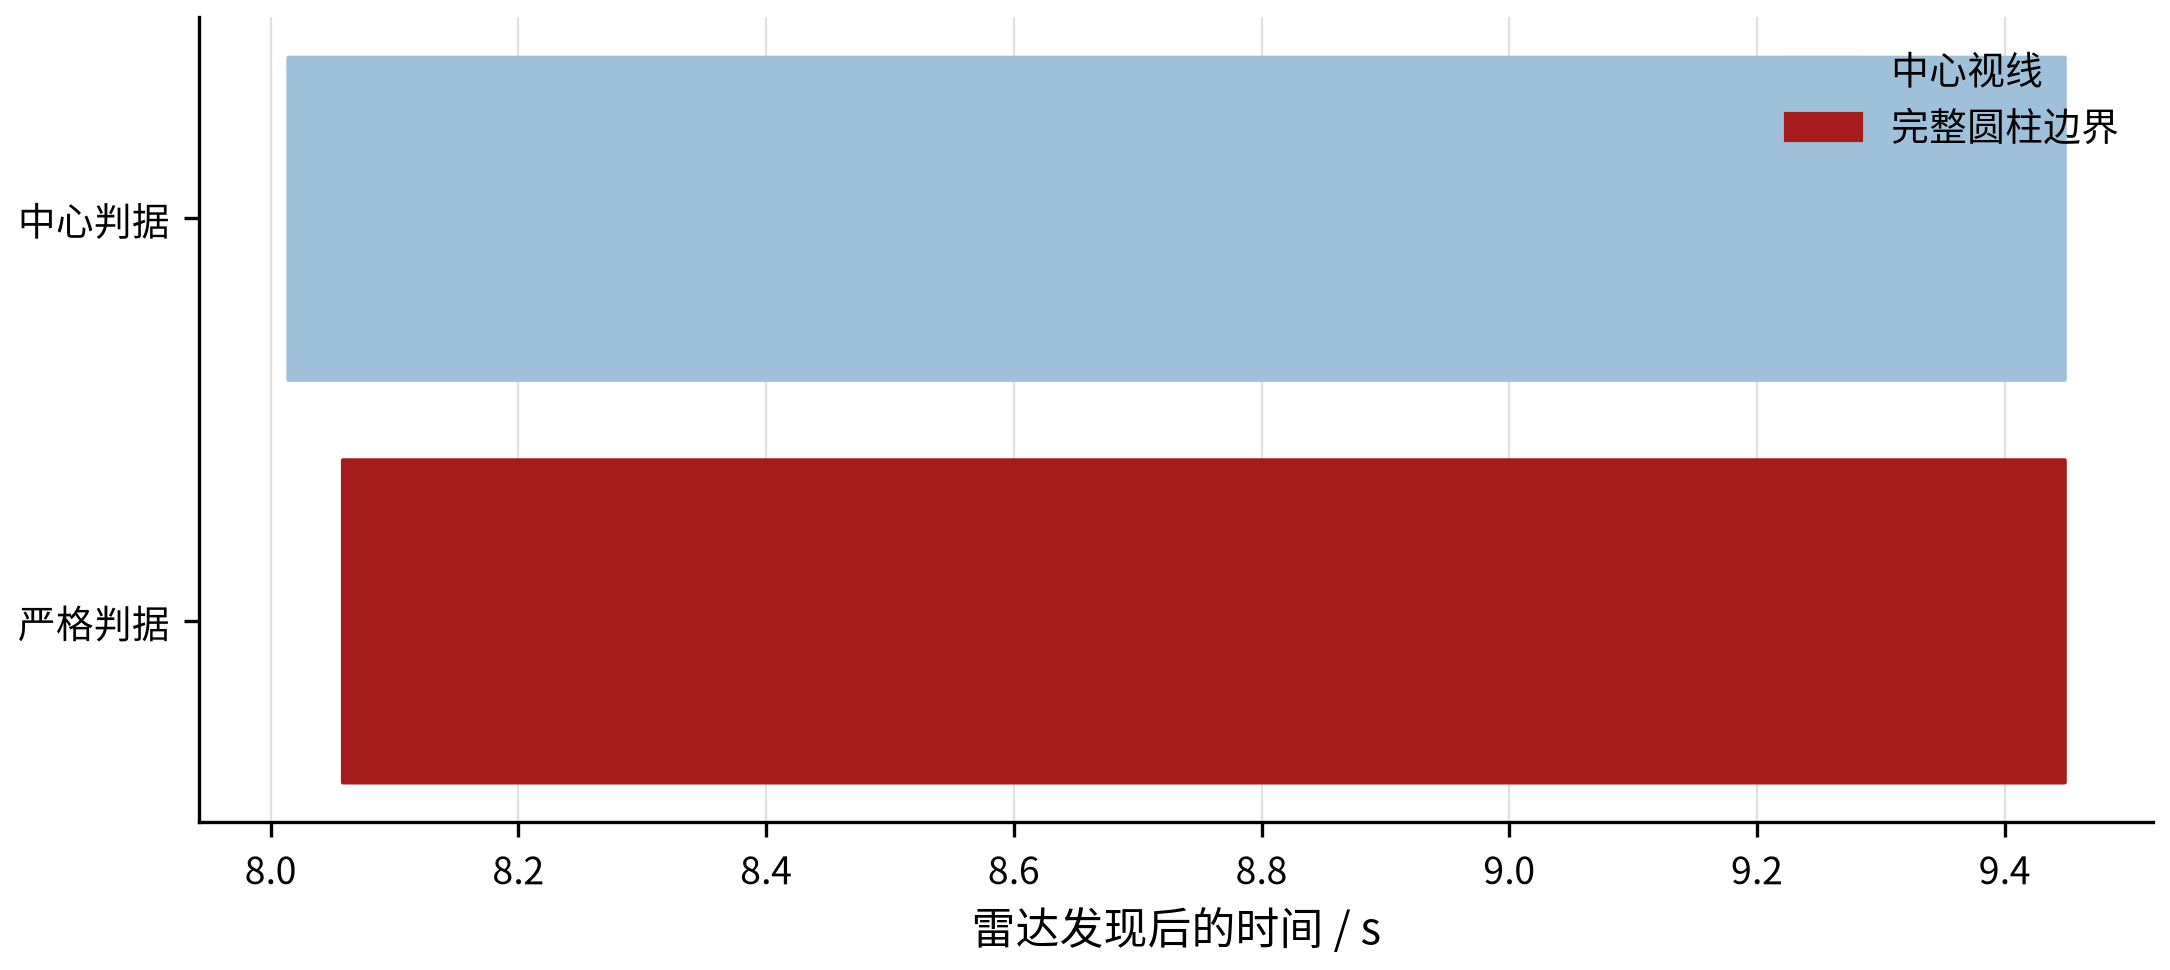
\includegraphics[width=0.78\textwidth]{fig1_q1_timeline.png}
\caption{完整圆柱边界判据与中心视线判据的遮蔽区间对比}
\end{figure}

中心视线判据得到 1.435 s，比严格判据高 0.043 s。由于题目明确给出圆柱尺寸，后续均采用严格判据。

\section{问题二：单弹投放优化}

直接搜索航向、速度、投放时刻与延时会产生大量远离视线的零适应度解。为缩小可行域，先选定期望遮蔽时刻 $t^*$、云团已形成时间 $a$ 和视线比例 $\lambda$，令期望云团中心位于
\begin{equation}
\boldsymbol q=\boldsymbol m_1(t^*)+\lambda[\boldsymbol o-\boldsymbol m_1(t^*)],
\end{equation}
其中 $\boldsymbol o=(0,200,5)$ 为目标中心。起爆点为 $\boldsymbol q+(0,0,3a)$，由其水平位移反算航向与速度，由高度差反算引信延时，再用差分进化优化三个参数。

\begin{table}[!htbp]
\centering\small
\caption{问题二最优单弹策略}
\begin{tabular}{cccccc}
\toprule
航向/$^\circ$ & 速度/(m/s) & 投放时刻/s & 起爆时刻/s & 起爆高度/m & 遮蔽时长/s \\
\midrule
176.91 & 71.00 & 0.009 & 2.461 & 1770.52 & 4.540 \\
\bottomrule
\end{tabular}
\end{table}

该策略的投放点为 $(17799.39,\,0.03,\,1800.00)$，起爆点为 $(17625.50,\,9.41,\,1770.52)$，遮蔽区间为 2.798--7.338 s。

\section{问题三与问题四：多弹协同}

\subsection{FY1 单机三弹}

无人机航向和速度固定不变。先求第一枚弹的可行视线参数解，再在同一航迹上枚举投放与延时组合，以新增遮蔽时间而不是单弹时长作为边际收益，并强制任意相邻投放时刻至少相隔 1 s。

\begin{table}[!htbp]
\centering\small
\caption{问题三 FY1 三弹投放策略}
\begin{tabular}{cccccc}
\toprule
弹号 & 航向/$^\circ$ & 速度/(m/s) & 投放时刻/s & 起爆时刻/s & 单弹时长/s \\
\midrule
1 & 178.43 & 80.74 & 0.66 & 3.58 & 4.52 \\
2 & 178.43 & 80.74 & 1.80 & 5.10 & 3.21 \\
3 & 178.43 & 80.74 & 3.00 & 6.90 & 0.70 \\
\bottomrule
\end{tabular}
\end{table}

三枚弹的联合遮蔽区间为 3.685--8.305 s，时长 4.620 s。单弹区间存在重叠，因此联合时长小于各弹时长之和。

\subsection{三机各投一弹}

对 FY1、FY2、FY3 的六种加入次序逐一搜索；每加入一架无人机，都以其相对已有方案的新增遮蔽测度为目标。

\begin{table}[!htbp]
\centering\small
\caption{问题四三架无人机协同策略}
\begin{tabular}{ccccccc}
\toprule
无人机 & 弹号 & 航向/$^\circ$ & 速度/(m/s) & 投放/s & 起爆/s & 单弹时长/s \\
\midrule
FY1 & 1 & 178.83 & 116.71 & 0.36 & 3.75 & 4.50 \\
FY2 & 1 & 272.41 & 137.53 & 3.71 & 9.82 & 3.91 \\
FY3 & 1 & 74.59 & 139.93 & 22.38 & 22.88 & 3.12 \\
\bottomrule
\end{tabular}
\end{table}

三架无人机产生三个互不重叠的有效区间，总时长 11.530 s，显著高于单机沿一条固定航迹投放三弹的结果。

\begin{figure}[!htbp]
\centering
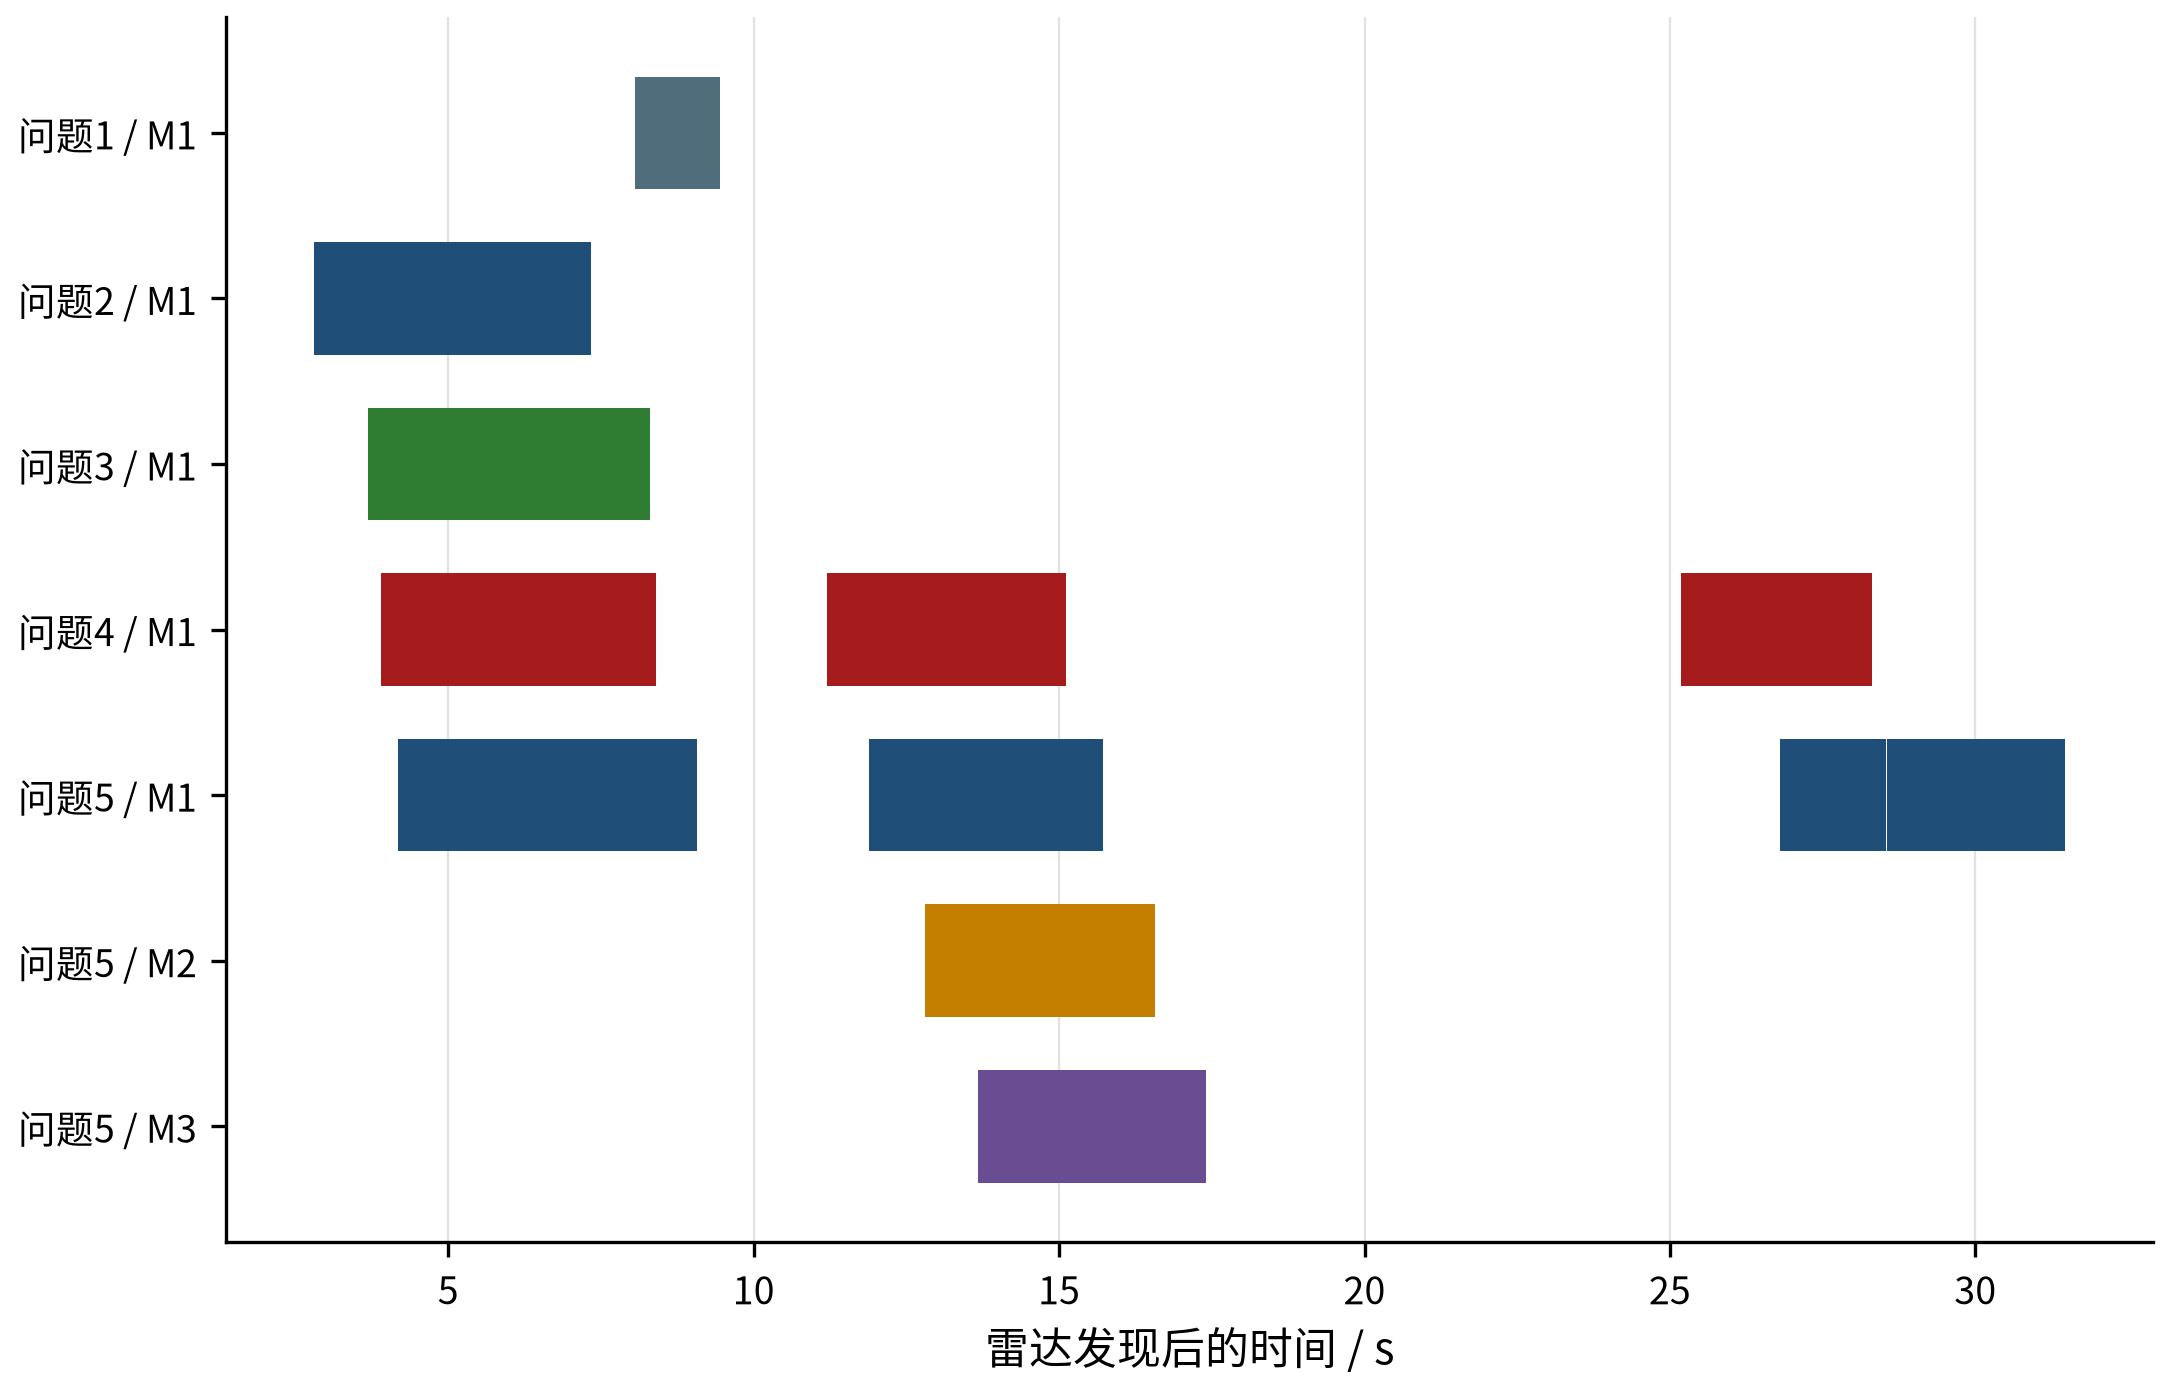
\includegraphics[width=0.86\textwidth]{fig2_intervals.png}
\caption{五个问题的有效遮蔽时间区间}
\end{figure}

\section{问题五：五机三导联合策略}

首先分别评估每个无人机--导弹组合的单弹可达遮蔽时长，在保证三枚导弹均获分配的条件下枚举 $3^5$ 种无人机任务组合；随后按边际收益安排同航迹追加弹。题设规定每架无人机至多投放 3 枚，因此仅保留产生正收益的弹，而不为填满表格安排无效投放。

\begin{table}[!htbp]
\centering\zihao{-5}
\caption{问题五实际采用的投放策略}
\begin{tabular}{cccccccc}
\toprule
无人机 & 弹号 & 航向/$^\circ$ & 速度/(m/s) & 投放/s & 起爆/s & 单弹时长/s & 导弹 \\
\midrule
FY1 & 1 & 178.93 & 103.55 & 0.71 & 4.05 & 4.50 & M1 \\
FY1 & 2 & 178.93 & 103.55 & 1.80 & 5.40 & 2.87 & M1 \\
FY1 & 3 & 178.93 & 103.55 & 3.00 & 7.20 & 1.10 & M1 \\
FY2 & 1 & 249.70 & 133.75 & 3.73 & 10.72 & 3.84 & M1 \\
FY2 & 2 & 249.70 & 133.75 & 4.80 & 11.10 & 1.74 & M1 \\
FY3 & 1 & 95.69 & 123.69 & 20.34 & 25.16 & 2.92 & M1 \\
FY4 & 1 & 285.67 & 139.27 & 1.54 & 11.89 & 3.77 & M2 \\
FY5 & 1 & 115.93 & 133.79 & 12.53 & 13.38 & 3.73 & M3 \\
\bottomrule
\end{tabular}
\end{table}

最终 FY1、FY2、FY3 共同干扰 M1，FY4 干扰 M2，FY5 干扰 M3。M1 的联合遮蔽时间为 13.400 s，M2 为 3.770 s，M3 为 3.730 s，总和 20.900 s。策略平面投影见图~\ref{fig:q5}，完整坐标见官方模板 \texttt{result3.xlsx}。

\begin{figure}[!htbp]
\centering
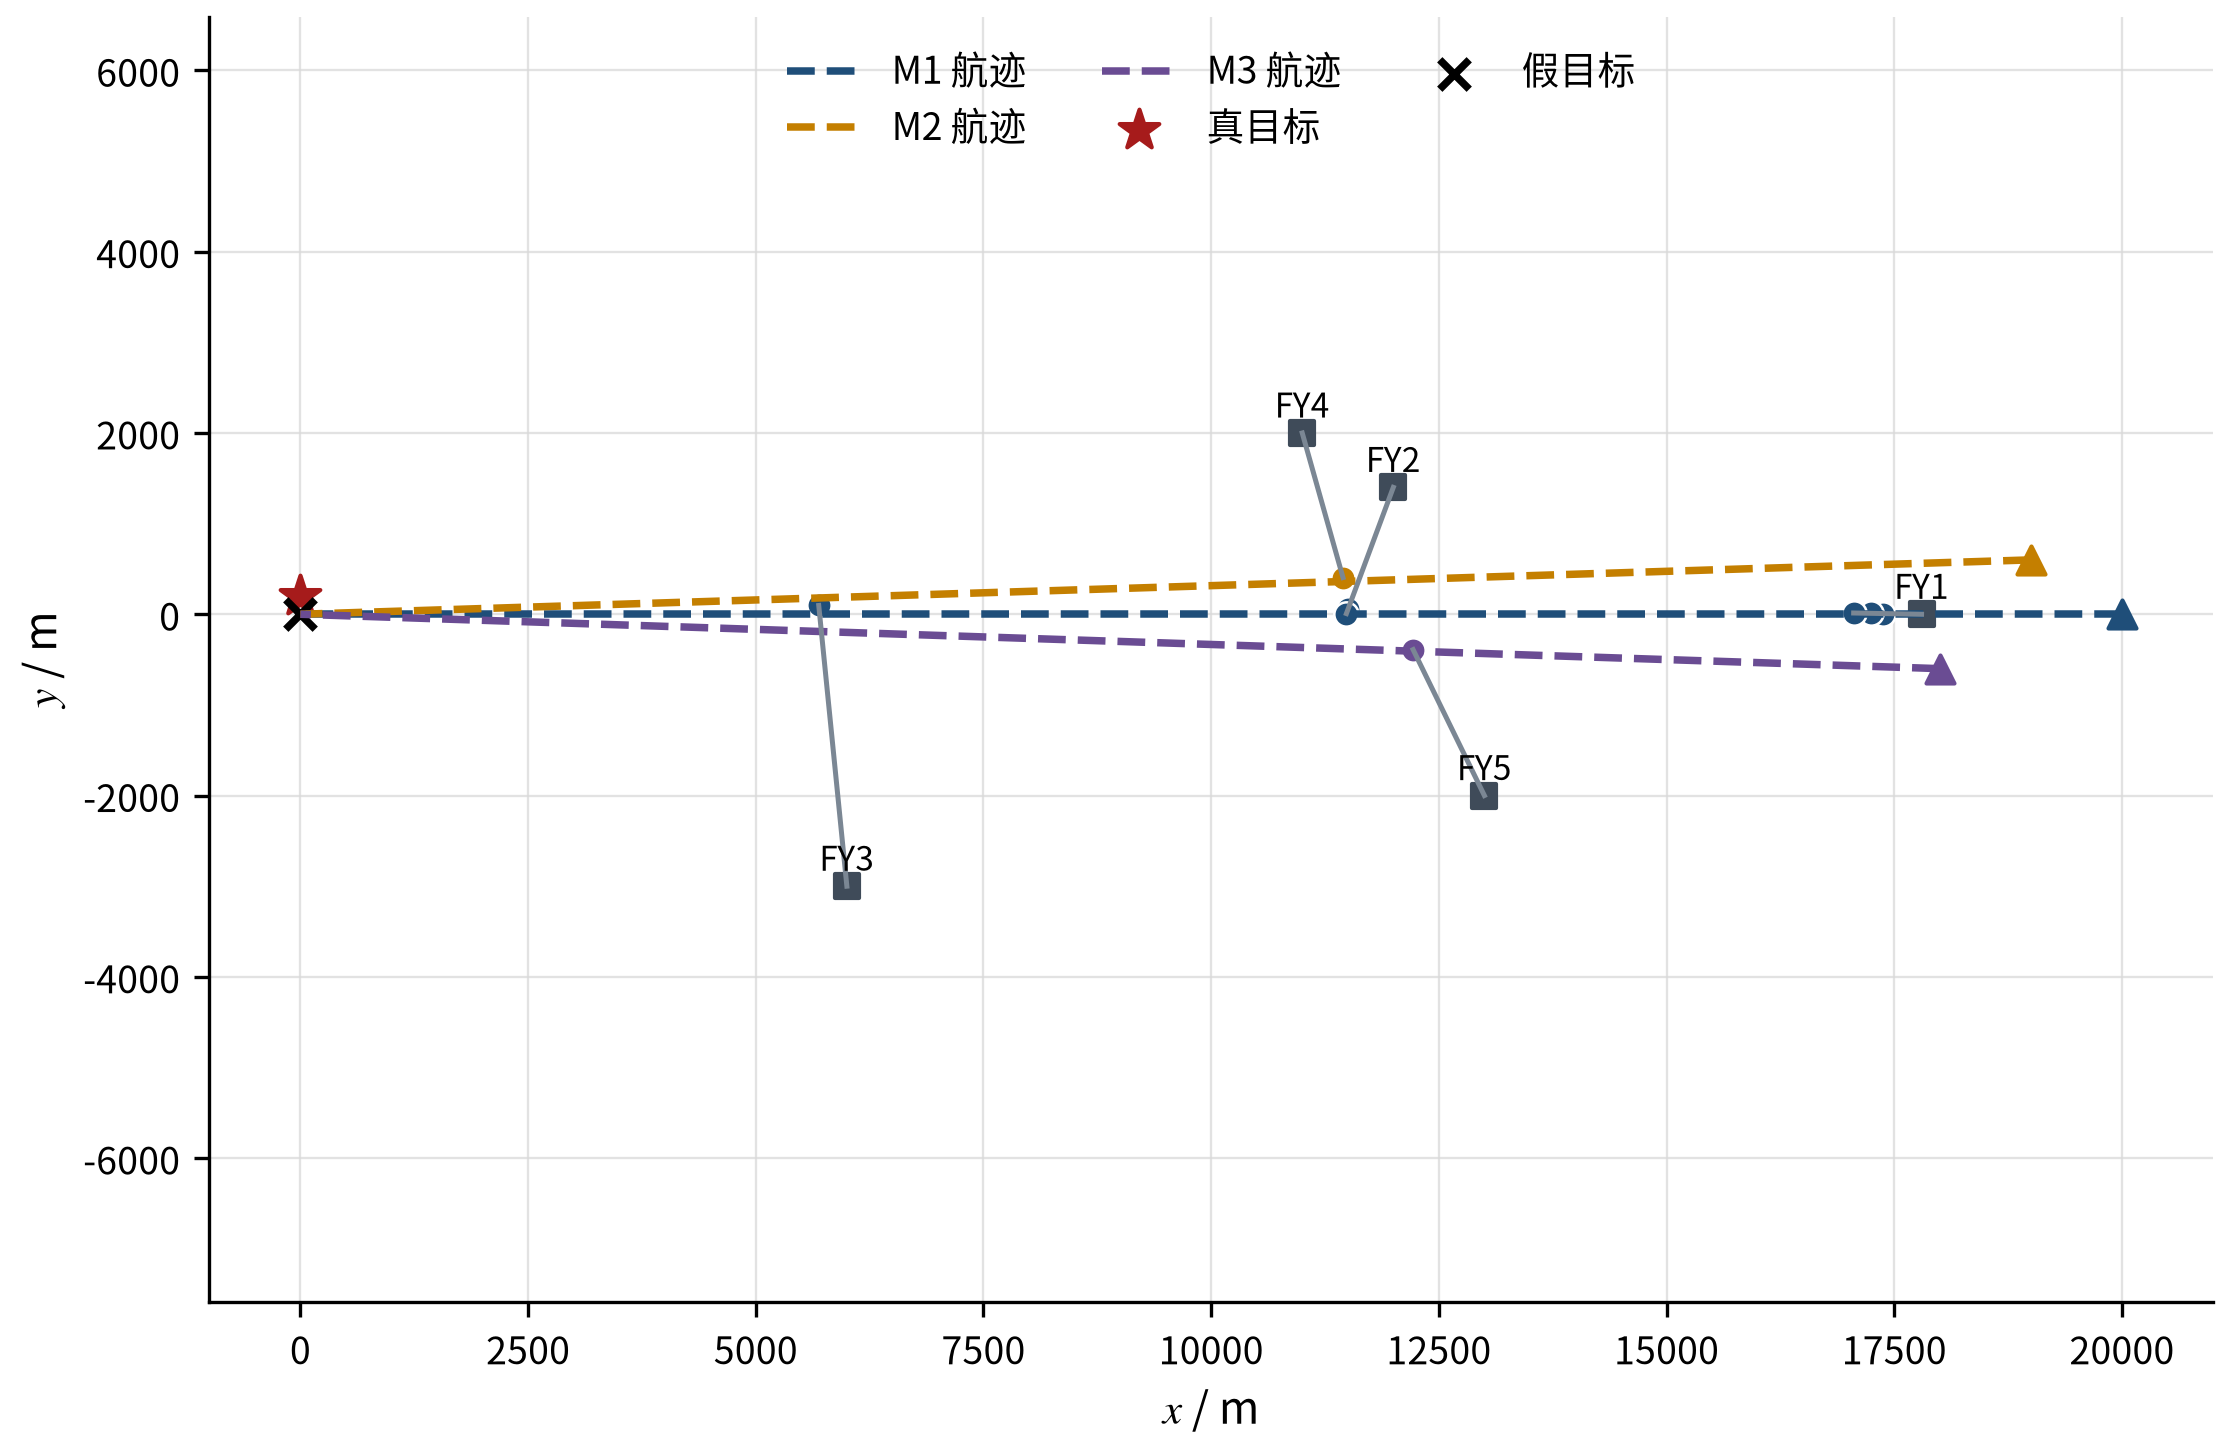
\includegraphics[width=0.90\textwidth]{fig3_q5_topview.png}
\caption{问题五导弹航迹、无人机航迹与烟幕起爆点平面投影}
\label{fig:q5}
\end{figure}

\section{精度与稳健性分析}

空间离散只取圆柱上下圆周的极值边界，逐步提高每个圆周采样数；时间离散则由 0.05 s 加密至 0.001 s。图~\ref{fig:resolution}表明问题一遮蔽时长趋于稳定，最终结果采用每圆周 360 点和 0.001 s 步长；优化问题复核采用每圆周 144 点和 0.005--0.01 s 步长。

\begin{figure}[!htbp]
\centering
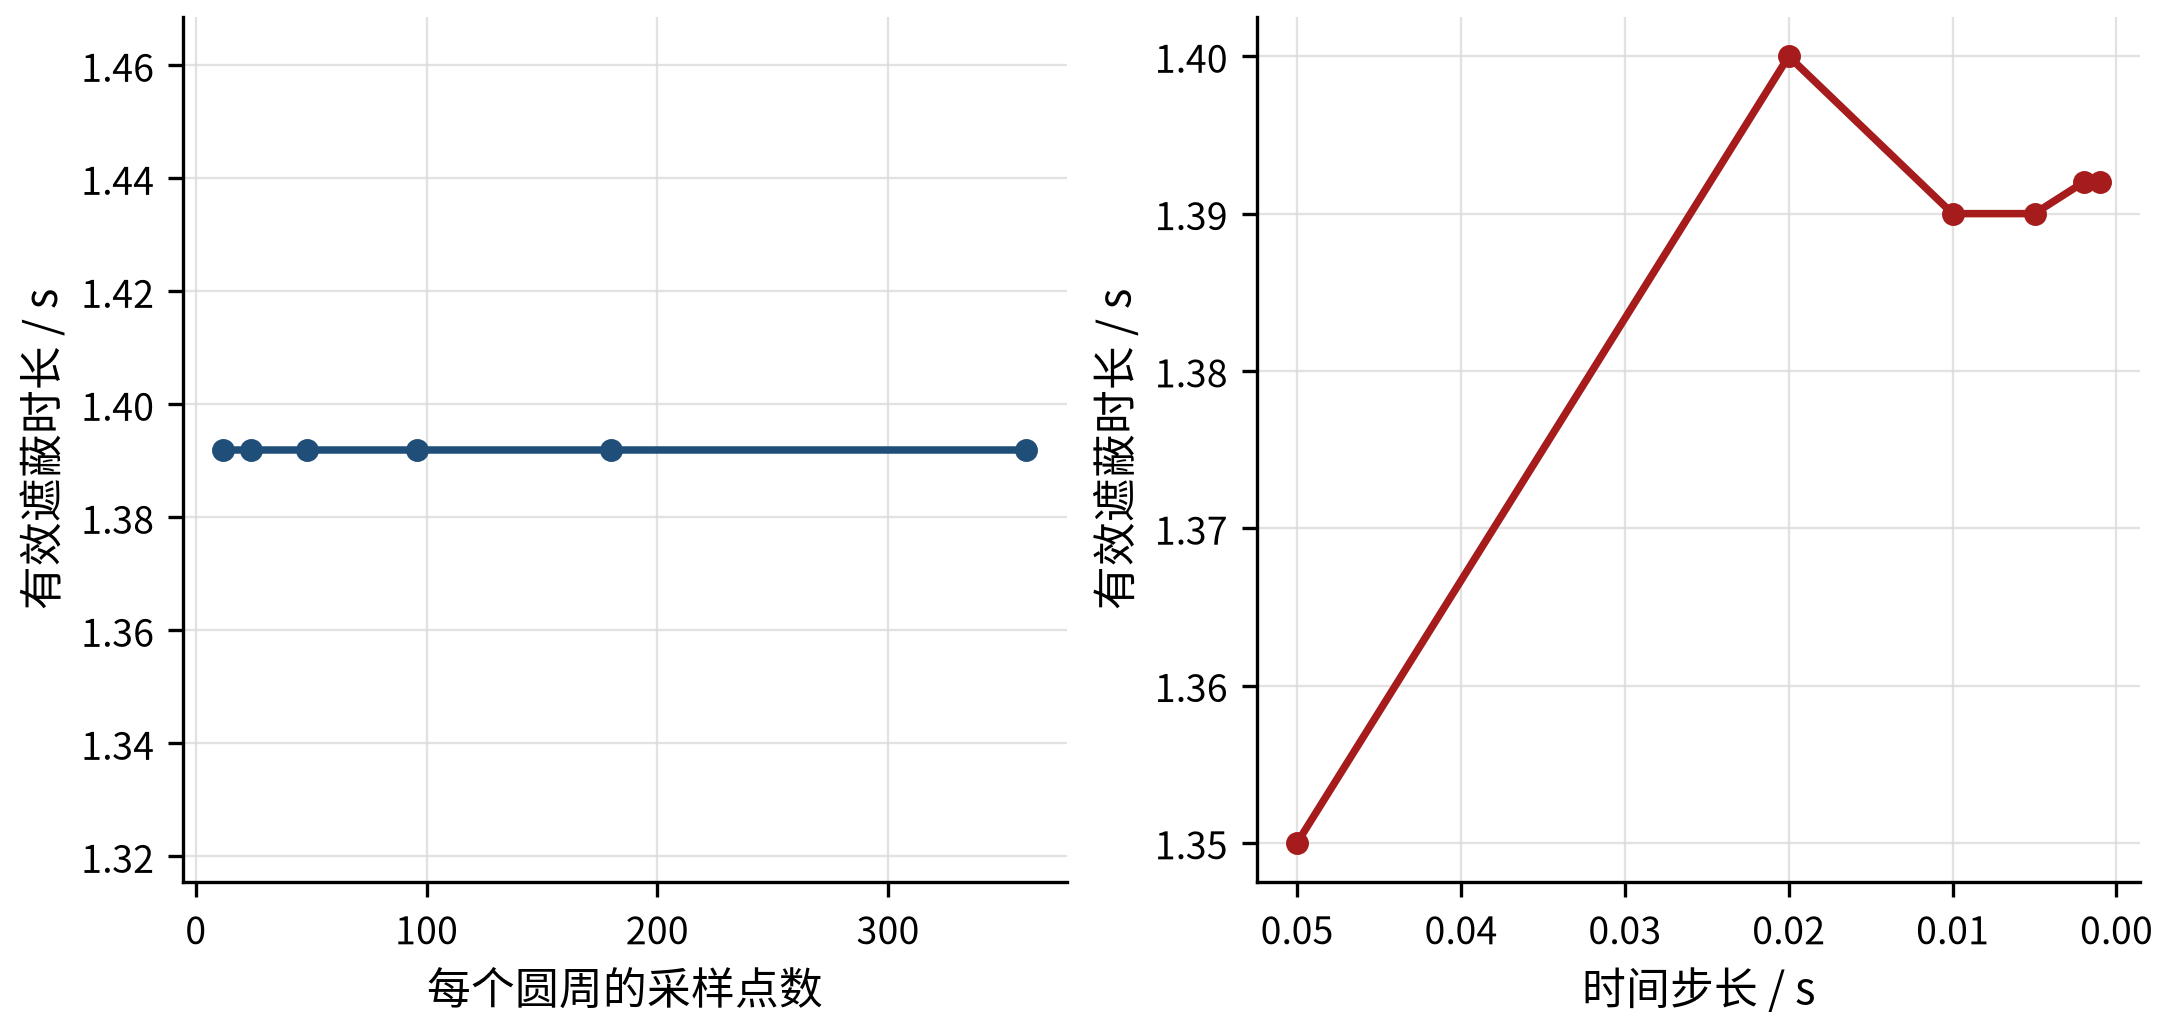
\includegraphics[width=0.84\textwidth]{fig4_resolution.png}
\caption{圆周采样数与时间步长的收敛性检查}
\label{fig:resolution}
\end{figure}

问题一的中心视线与完整边界结果相差 0.043 s，说明结论对遮蔽定义存在可解释的模型敏感性。本文采用更保守的完整边界口径，故所有工作簿中的有效时长均未使用中心线近似。

\section{模型评价与推广}

\subsection{模型的优点}
\begin{enumerate}
  \item 运动方程直接对应题设物理阶段，所有投放点和起爆点可由统一时钟复算；
  \item 完整边界判据利用了圆柱尺寸，并通过独立的线段--球二次方程交叉验证；
  \item 多弹目标使用时间集合并集，避免重叠时长重复累加；
  \item 视线参数化使搜索集中在几何可行区域，固定种子可复现实验结果。
\end{enumerate}

\subsection{模型的局限}
\begin{enumerate}
  \item 未考虑风、空气阻力、云团扩散和浓度随时间衰减，实际应用需引入随机风场；
  \item 圆柱边界采用有限采样，虽已做收敛检查，仍属于数值近似；
  \item 问题五采用分层配对和贪心追加，而非对全部变量一次性全局优化，结果是可行优质解但不宣称严格全局最优；
  \item 将三枚导弹遮蔽时长之和作为目标，若任务要求三弹同时被遮蔽，应改为三个时间集合的交集测度。
\end{enumerate}

\begin{thebibliography}{9}
\bibitem{problem} 全国大学生数学建模竞赛组委会. 2025 年高教社杯全国大学生数学建模竞赛 A 题[EB/OL]. 2025-09-04.
\bibitem{de} Storn R, Price K. Differential Evolution--A Simple and Efficient Heuristic for Global Optimization over Continuous Spaces[J]. Journal of Global Optimization, 1997, 11: 341--359.
\bibitem{scipy} Virtanen P, et al. SciPy 1.0: Fundamental Algorithms for Scientific Computing in Python[J]. Nature Methods, 2020, 17: 261--272.
\bibitem{ai-codex} OpenAI. Codex CLI, 0.146.0, OpenAI, 使用日期: 2026-08-02.
\end{thebibliography}

\begin{aideclaration}[AI 工具使用声明]
本次模拟使用 OpenAI Codex 协助搭建程序结构、执行数值试验和整理论文文字。运动方程、几何判据、约束审计和全部数值均由本目录代码重新计算；正式参赛时应由参赛队员独立复核模型选择、程序实现与结果解释。
\end{aideclaration}

\par\medskip
\noindent\textbf{支撑文件：}
\texttt{model.py}（运动与遮蔽判定），
\texttt{solve.py}（优化与工作簿填写）。
\par\noindent
\texttt{output/results.json}（完整数值结果）；
\texttt{result1.xlsx}、\texttt{result2.xlsx}、
\texttt{result3.xlsx}（官方模板结果，均位于 \texttt{output/}）。

\end{document}
